%\documentclass[tikz,crop,convert={density=200,outext=.png},border=0.4cm,width=6cm,height=3cm]{standalone}
\documentclass[tikz,border=0.3cm]{standalone}
\usepackage[left=2.2cm,right=2.2cm,top=2.5cm,bottom=2.0cm,a4paper]{geometry}
\usepackage{pgfplots}
\usepackage{amsmath}
\usetikzlibrary{arrows.meta}
\usepackage{physics}
\pgfplotsset{compat=newest,
    %width=6cm,
    %height=3cm,
    scale only axis=true,
    max space between ticks=25pt,
    try min ticks=5,
    every axis/.style={
        axis y line=middle,
        axis x line=middle,
        axis line style={thick,->,>=latex, shorten >=-.3cm}
    },
      every axis plot/.append style={thick},
    tick style={black, thick},
}
\tikzset{
    semithick/.style={line width=0.8pt},
}
\usepgfplotslibrary{groupplots}
\usepgfplotslibrary{dateplot}
\usetikzlibrary{positioning}
%\pgfplotsset{compat=1.17}

\begin{document}
\begin{tikzpicture}
\node[inner sep=0pt] (mixed) at (-5,0)
{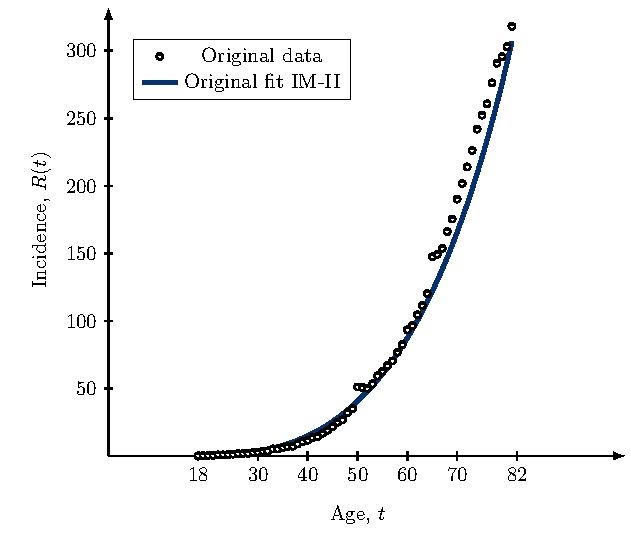
\includegraphics[width=0.3\textwidth]{original_fit.pdf}};
\node[inner sep=0pt] (power_law) at (0,0)
{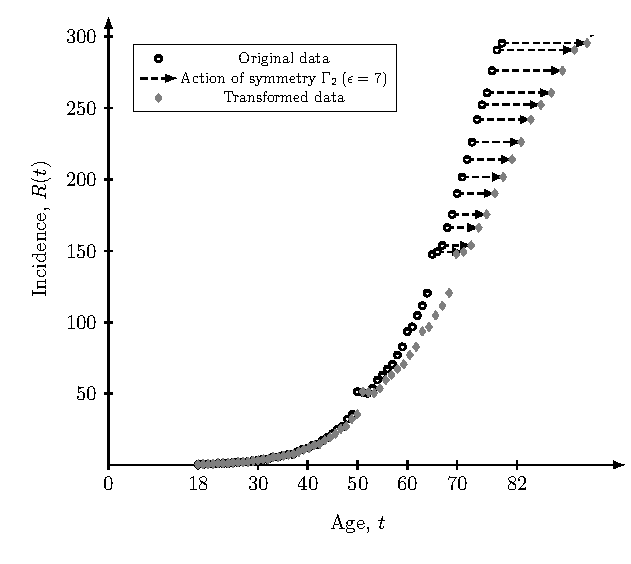
\includegraphics[width=0.3\textwidth]{transform_data.pdf}};
  \node[inner sep=0pt] (exponential) at (5,0)
    {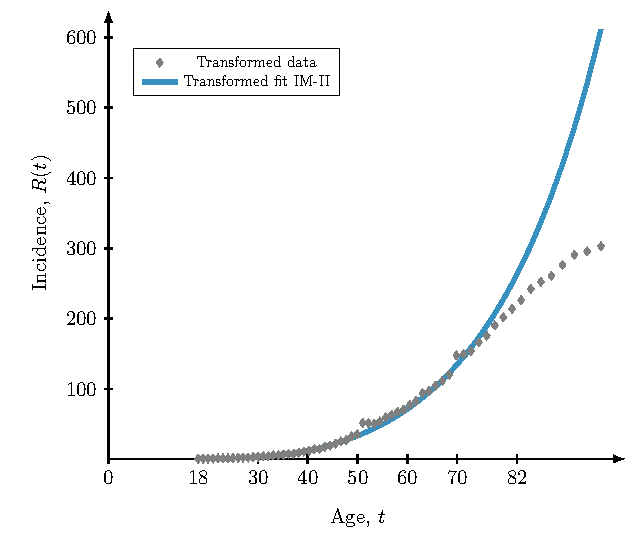
\includegraphics[width=0.3\textwidth]{transformed_fit.pdf}};

\node (b) at (-2.12,2.5) {(\textbf{B})};
\node[left=4.2cm of b] (a) {(\textbf{A})};
\node[right=4.2cm of b] (c) {(\textbf{C})};
%\draw (-2.35,-4) -- (-2.35,4);
\end{tikzpicture}

\end{document}
